
\section{Humanoid Robots}
Humanoid Robots are robotic mechanisms resembling the kinematics of human beings with a head and a torso bridging two arms \& two legs. There are many variants modeling only certain parts of the human body though we stick with the context of legged robots with arms through out this report. Building humanoid robots require the need of understanding human behaviors and kinematic structure deeply. Attempting to build such robots sometimes give us better understanding of human beings making the knowledge flow between both the domains bi-directional. The anthropomorphic design of humanoids also help in getting the acceptance of people as a social entity making the human-robot interaction feasible \cite{fink2012anthropomorphism}. Also the physical ability of humanoids make them suitable for rescue or disaster handling scenarios. The social acceptance and the physical ability of humanoids make them a very good platform to invest on researching technologies that improve the intelligence of such robots.

\subsection{History of Humanoid Robots}
Humanoid robots were just controlled using traditional joint position control methodologies like in industrial robots though there is a need for stiff drive train for precision. WABOT-1 was the first humanoid robot to walk, communicate, visually recognize objects and manipulate them. The robot was built by Kato's lab from University of Waseda in 1973 \cite{kato1973development}. The same lab lead a series of developments achieving the latest one WABIAN-2 which can walk with stretched knees \cite{ogura2006development}. Chronologically WABOT-1 was followed by P2, the first robot to perform stable walking, was launched in 1996 by Honda after 10 years of modular and systematic research focused on dynamic biped walking and stability control \cite{hirai1998development}. The next version P3  was much lighter and gave way to the launch of the famous ASIMO robot in 2000 with a more friendly appearance and improved intelligence \cite{hirose2007honda}. ASIMO's impressive capabilities attracted the attention of robotics researchers and created a perspective of humanoid robots to be exploited for service robotics \cite{kaneko2009cybernetic}. 


\begin{figure}[!tbph]
\begin{subfigure}
[WABOT-1]{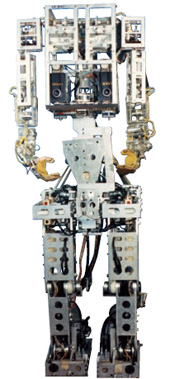
\includegraphics[width=4.1cm,height=6cm]{chapters/intro/images/wabot1.jpg}}\quad
\end{subfigure}
\begin{subfigure}
[ASIMO]{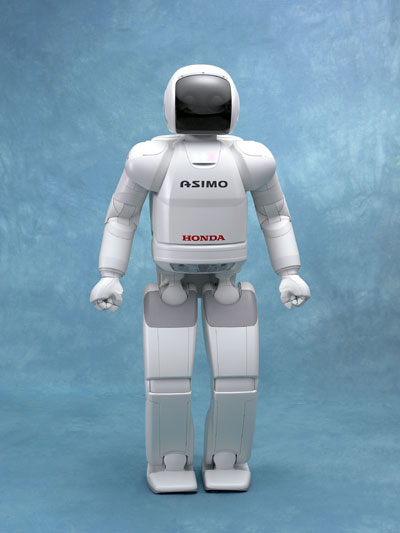
\includegraphics[width=4.2cm,height=6cm]{chapters/intro/images/asimo.jpg}}\quad
\end{subfigure}
\begin{subfigure}
[Kobian]{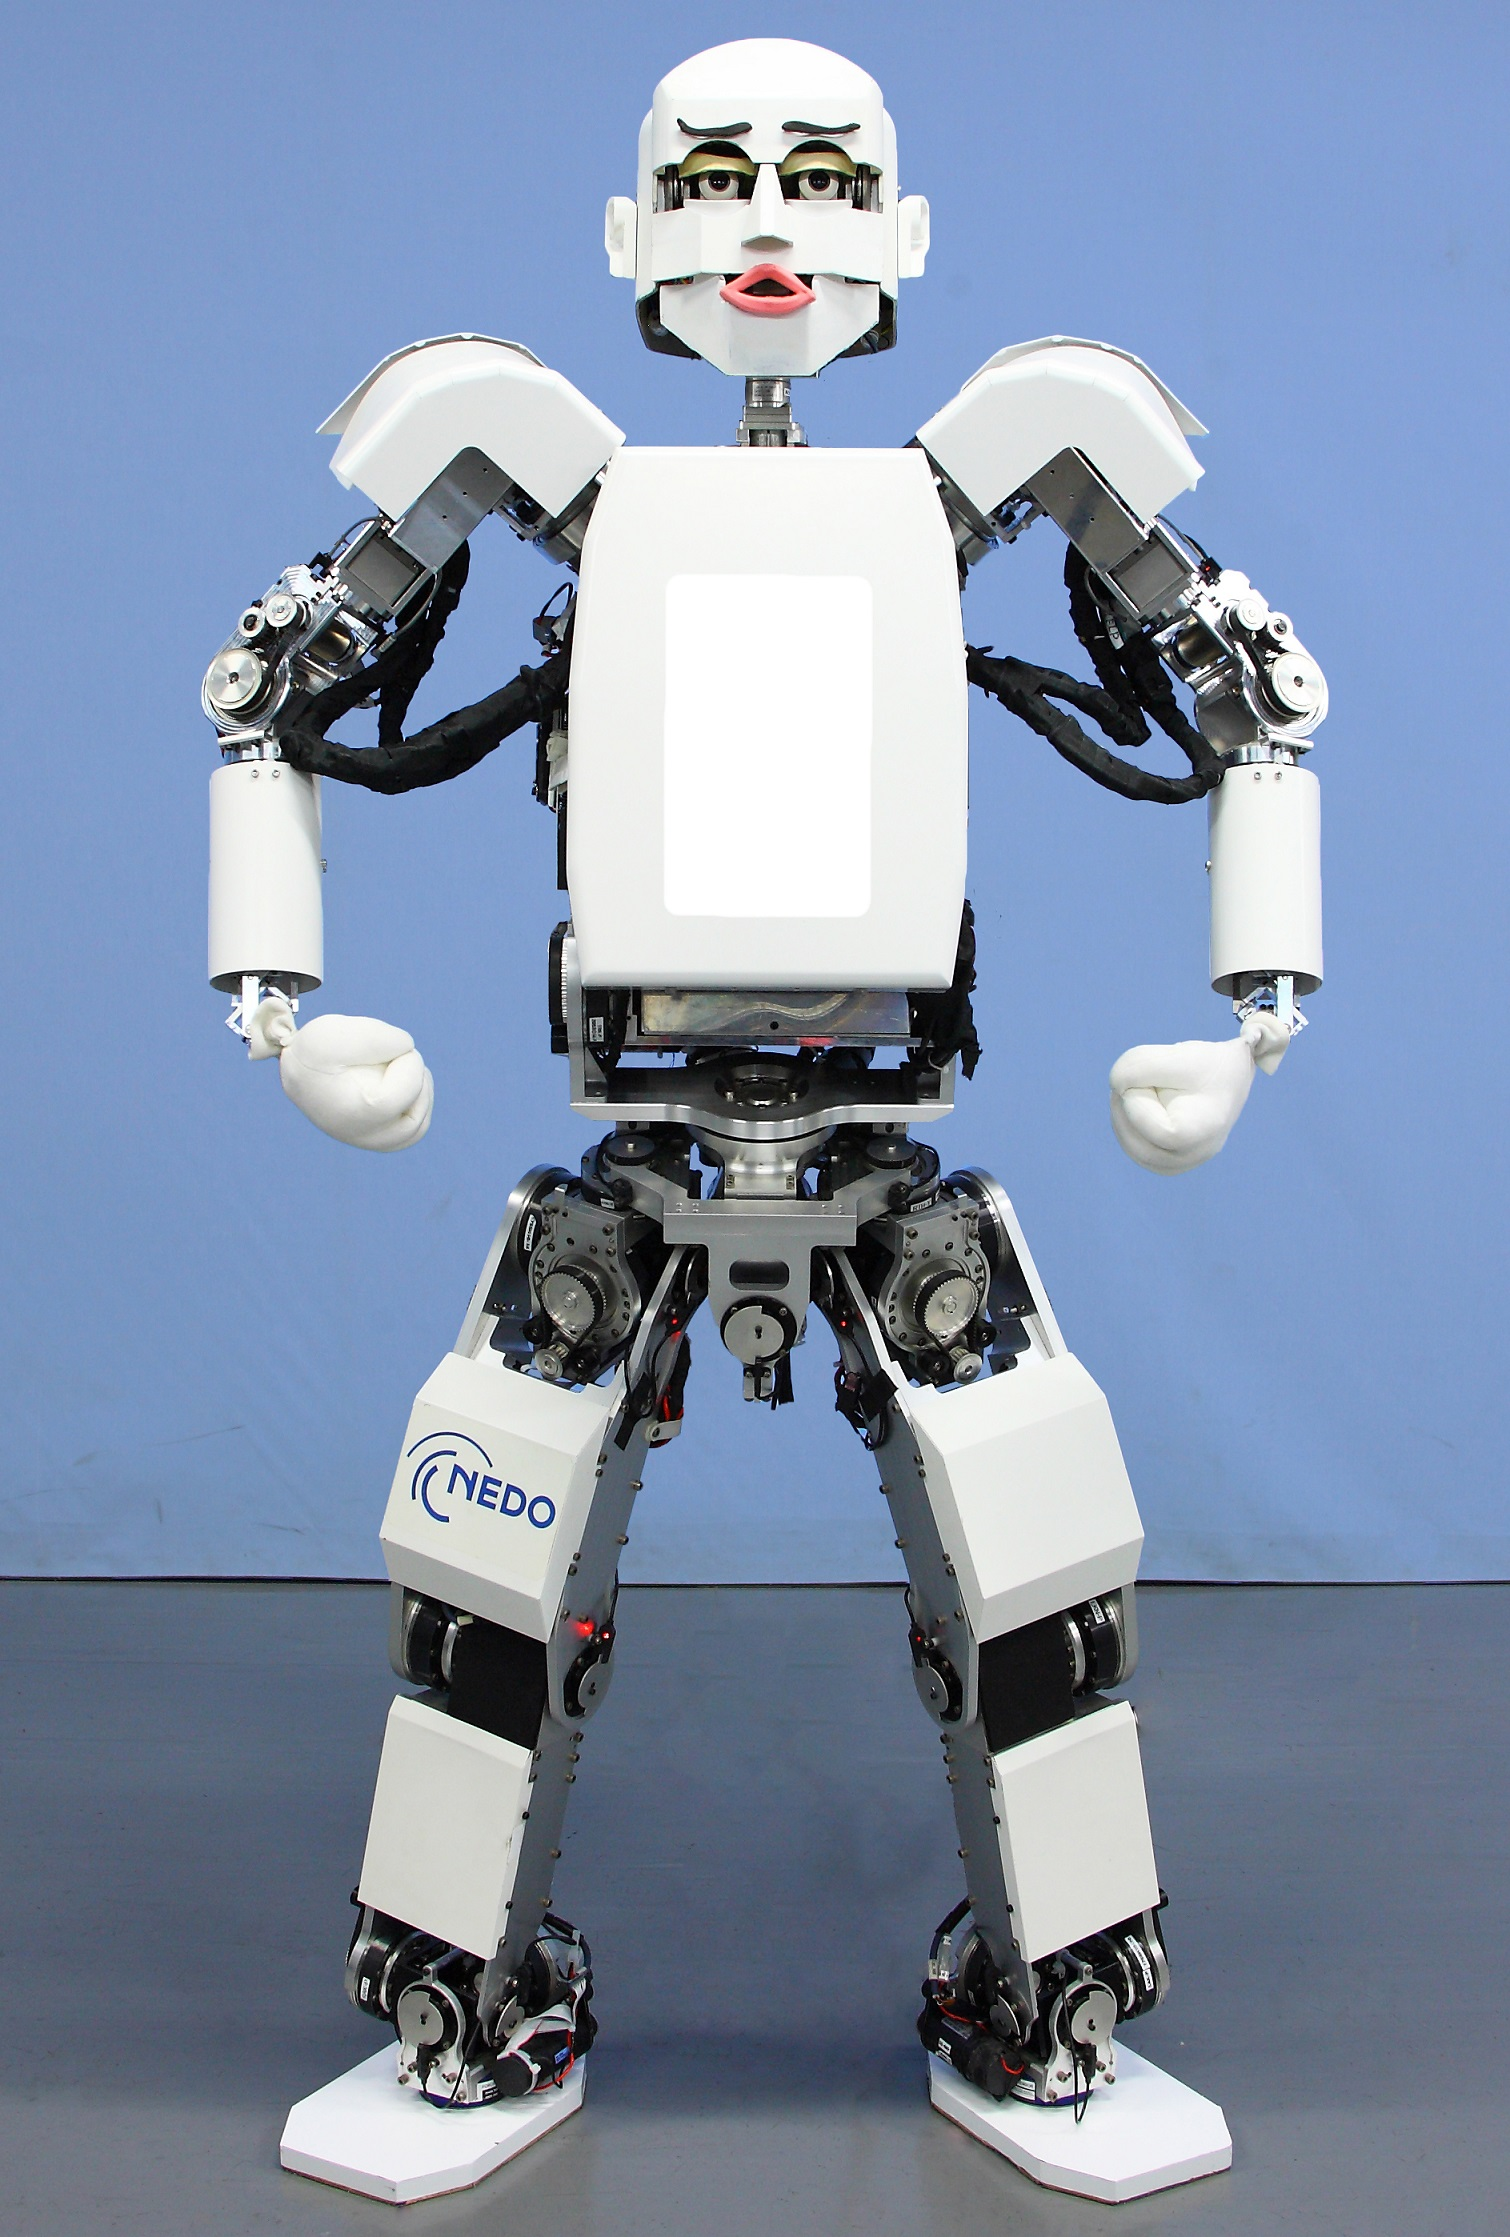
\includegraphics[width=4.2cm,height=6cm]{chapters/intro/images/kobian.jpg}}\quad
\end{subfigure}
\caption{Humanoids of the first generation}
\label{fig:hr_first}
\end{figure}


Japan took the trigger seriously and many humanoids were developed in the last decade both for entertainment and demonstrating physical capabilities. Different sized humanoids with great capabilities were built within the \textit{Humanoid Robotics Project} by Kawada Industries and Japanese National Institute of Advanced Industrial Science and Technology (AIST)  with the first prototype HRP-2P launched in 2002 \cite{kaneko2002design} followed by HRP-2 \cite{Kaneko04humanoidrobot}, HRP-3 \cite{kaneko2008humanoid} in the next years. HRP-4C in 2009 \cite{kaneko2009cybernetic}, assumes a feminine appearance while the latest HRP4 in 2010, is more athletic and light \cite{kaneko2011humanoid}. Sony launched QRIO (previously called SDR-3X), a small humanoid robot for entertainment in 2004 \cite{geppert2004qrio}. Fujitsu Automation also launched a series of small humanoid robots HOAP with the latest version HOAP-3 released in 2005. Other japanese robots include H7  from the University of Tokyo \cite{nishiwaki2007experimental}, Kenta, a musculo-skeletal robot \cite{inaba2003building}, Kojiro in 2007 \cite{mizuuchi2007advanced},Kenshiro in 2012 \cite{nakanishi2012design}. Schaft launched one of the most powerful humanoid robots inspired from HRP-2 series robots in 2013.

The Korea Advanced Institute of Science and Technology (KAIST) invested in developing several versions of KAIST humanoid robots(KHR) since 2002 with the latest one released in 2011 with the name HUBO 2 \cite{kim2002development,park2005mechanical,park2005development,grey2013multi}. The other well known network based robots from Korea are the MAHRU and AHRA series \cite{you2005network,kwon2007biped, kim2011providing}. Technical Unversity of Munich (TUM) built the humanoid robot Johnnie \cite{gienger1999design} followed by an improved version called Lola \cite{lohmeier2009humanoid} known for its fast and robust motions. The Italian Institute of Technology (IIT)  built a torque controlled iCub \cite{metta2010icub} and COMAN in 2012
\cite{tsagarakis2013compliant}. The University Carlos III from Spain, built the Rh-1 in 2007 \cite{arbulu2007real} and its successor TEO in 2011 \cite{monje2011full}. Pal Robotics also built the humanoid robots REEM-B \cite{tellez2008reem}, REEM-C, a human friendly design in 2014 \cite{robotics2014reem}. In 2007, Aldebaran Robotics, a french company launched Nao, one of the most popular small humanoid robot in the world motivated several laboratories to do research on humanoids with less investment \cite{gouaillier2009mechatronic}. The same company presented a torque controlled child-size robot Romeo. 

\begin{figure}[h]
\begin{subfigure}
[HRP2]{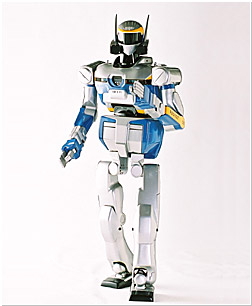
\includegraphics[width=4.4cm,height=6cm]{chapters/intro/images/hrp2.jpg}}\quad
\end{subfigure}
\begin{subfigure}
[Kojiro]{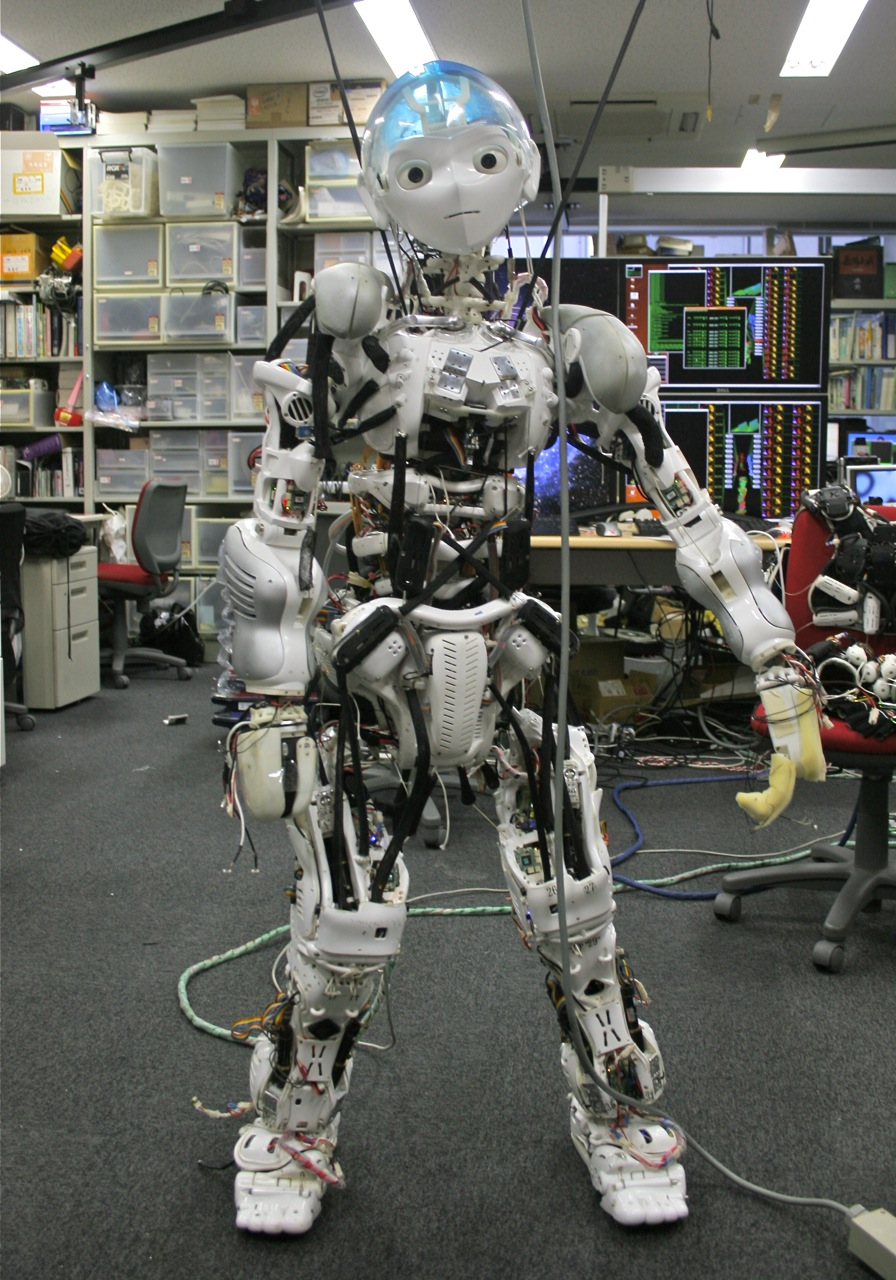
\includegraphics[width=4cm,height=6cm]{chapters/intro/images/kojiro.jpg}}\quad
\end{subfigure}
\begin{subfigure}
[Kenshiro]{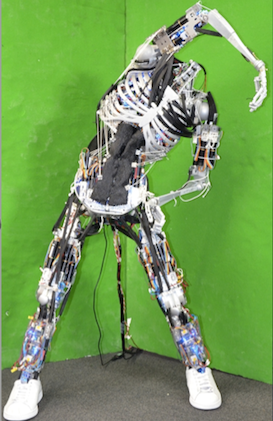
\includegraphics[width=4.1cm,height=6cm]{chapters/intro/images/kenshiro.png}}\quad
\end{subfigure}
\caption{Japanese Humanoids }
\label{fig:hr_second}
\end{figure}

SARCOS Research Corporation and ATR (Advanced Telecommunications Research Institute International) from Japan built robots Erato DB (Dynamic Brain) based on hydraulic actuation in 2000 \cite{atkeson2000using}, and CBi in 2006 \cite{cheng2007cb} which explores the background neural processes in the human brain. DARPA Robotics Challenge (DRC), a competition funded by US Defense Advanced Research Projects Agency (DARPA)  was held between 2012-2015 motivated the development of humanoid robots in the US.  CHARLI in 2010 \cite{knabe2013team}, THOR in 2014 \cite{yi2015team}, CHIMP in 2013 \cite{stentz2015chimp}, Valkyrie in 2013 \cite{radford2015valkyrie} are some popular robots in the US.Most of the robots presented above are fully actuated electrical systems which usually compose rigid bodies with compliance only in the foot to handle contact impacts from the ground while walking. Also they mostly use the traditional high-gain position control methodologies which requires a precise robot dynamic model and Zero Moment Point (ZMP) concept by Vukobratovic \cite{vukobratovic1972stability} is applied in the control of many bipeds \cite{hirai1998development,Kaneko04humanoidrobot,grey2013multi}. 

The advanced robots are expected to make intelligent interactions with the environment. Torque control has gained enough attention in the recent past for its ability to make robust and compliant interactions with the environment and human beings with greater agility and safety. Human safety is one crucial issue which doesn't allow service robots in mobile or humanoid form to be commercialized as domestic robots. Higher compliance brings automatic adaption to un-modeled and uncertain environments making the interaction safer than executing the traditional position control on robots. There are two main categories of torque control: Impedance control and Inverse dynamics control. Impedance Control \cite{part1985impedance,albu2007unified,ott2008passivity,schaffer2008soft} is known for its passivity properties very suitable for interaction with humans and unknown environments. Inverse dynamics(ID) control \cite{del2016implementing,buchli2009compliant,righetti2013optimal} is a highly complex technique which needs a dynamic model and joint torque measurements to control the interactions with the world. This technique provides good trajectory tracking and highly compliant behavior with low feedback gains. The new age ID controllers use quadratic programming(QP) solvers which allow to add constraints such as joint limits, torque bounds, contact force friction cones,center of pressure (CoP) limits which are crucial in humanoid robots. The interest in torque control of humanoid robots lead to new range of robots with torque sensing though it can be estimated in robots with no torques sensors as in HRP-2, iCub, HRP-4 and Asimo, etc.
\begin{figure}[!tbph]
\centering
\begin{subfigure}
[SARCOS]{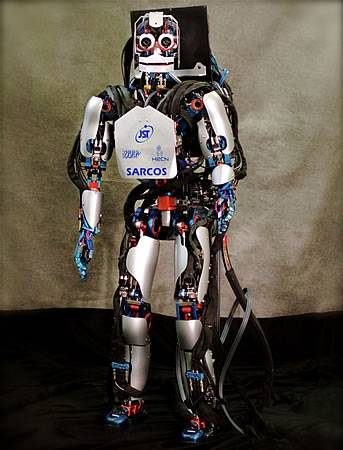
\includegraphics[width=4.2cm,height=6cm]{chapters/intro/images/sarcos.jpg}}\quad
\end{subfigure}
\begin{subfigure}
[CHIMP]{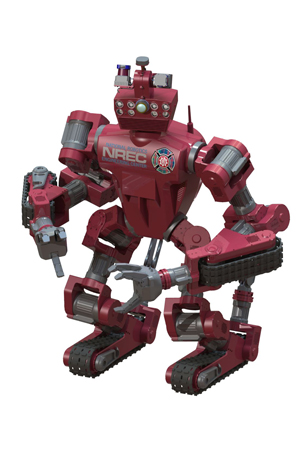
\includegraphics[width=4.2cm,height=6cm]{chapters/intro/images/chimp.jpg}}\quad
\end{subfigure}
\begin{subfigure}
[Valkyrie]{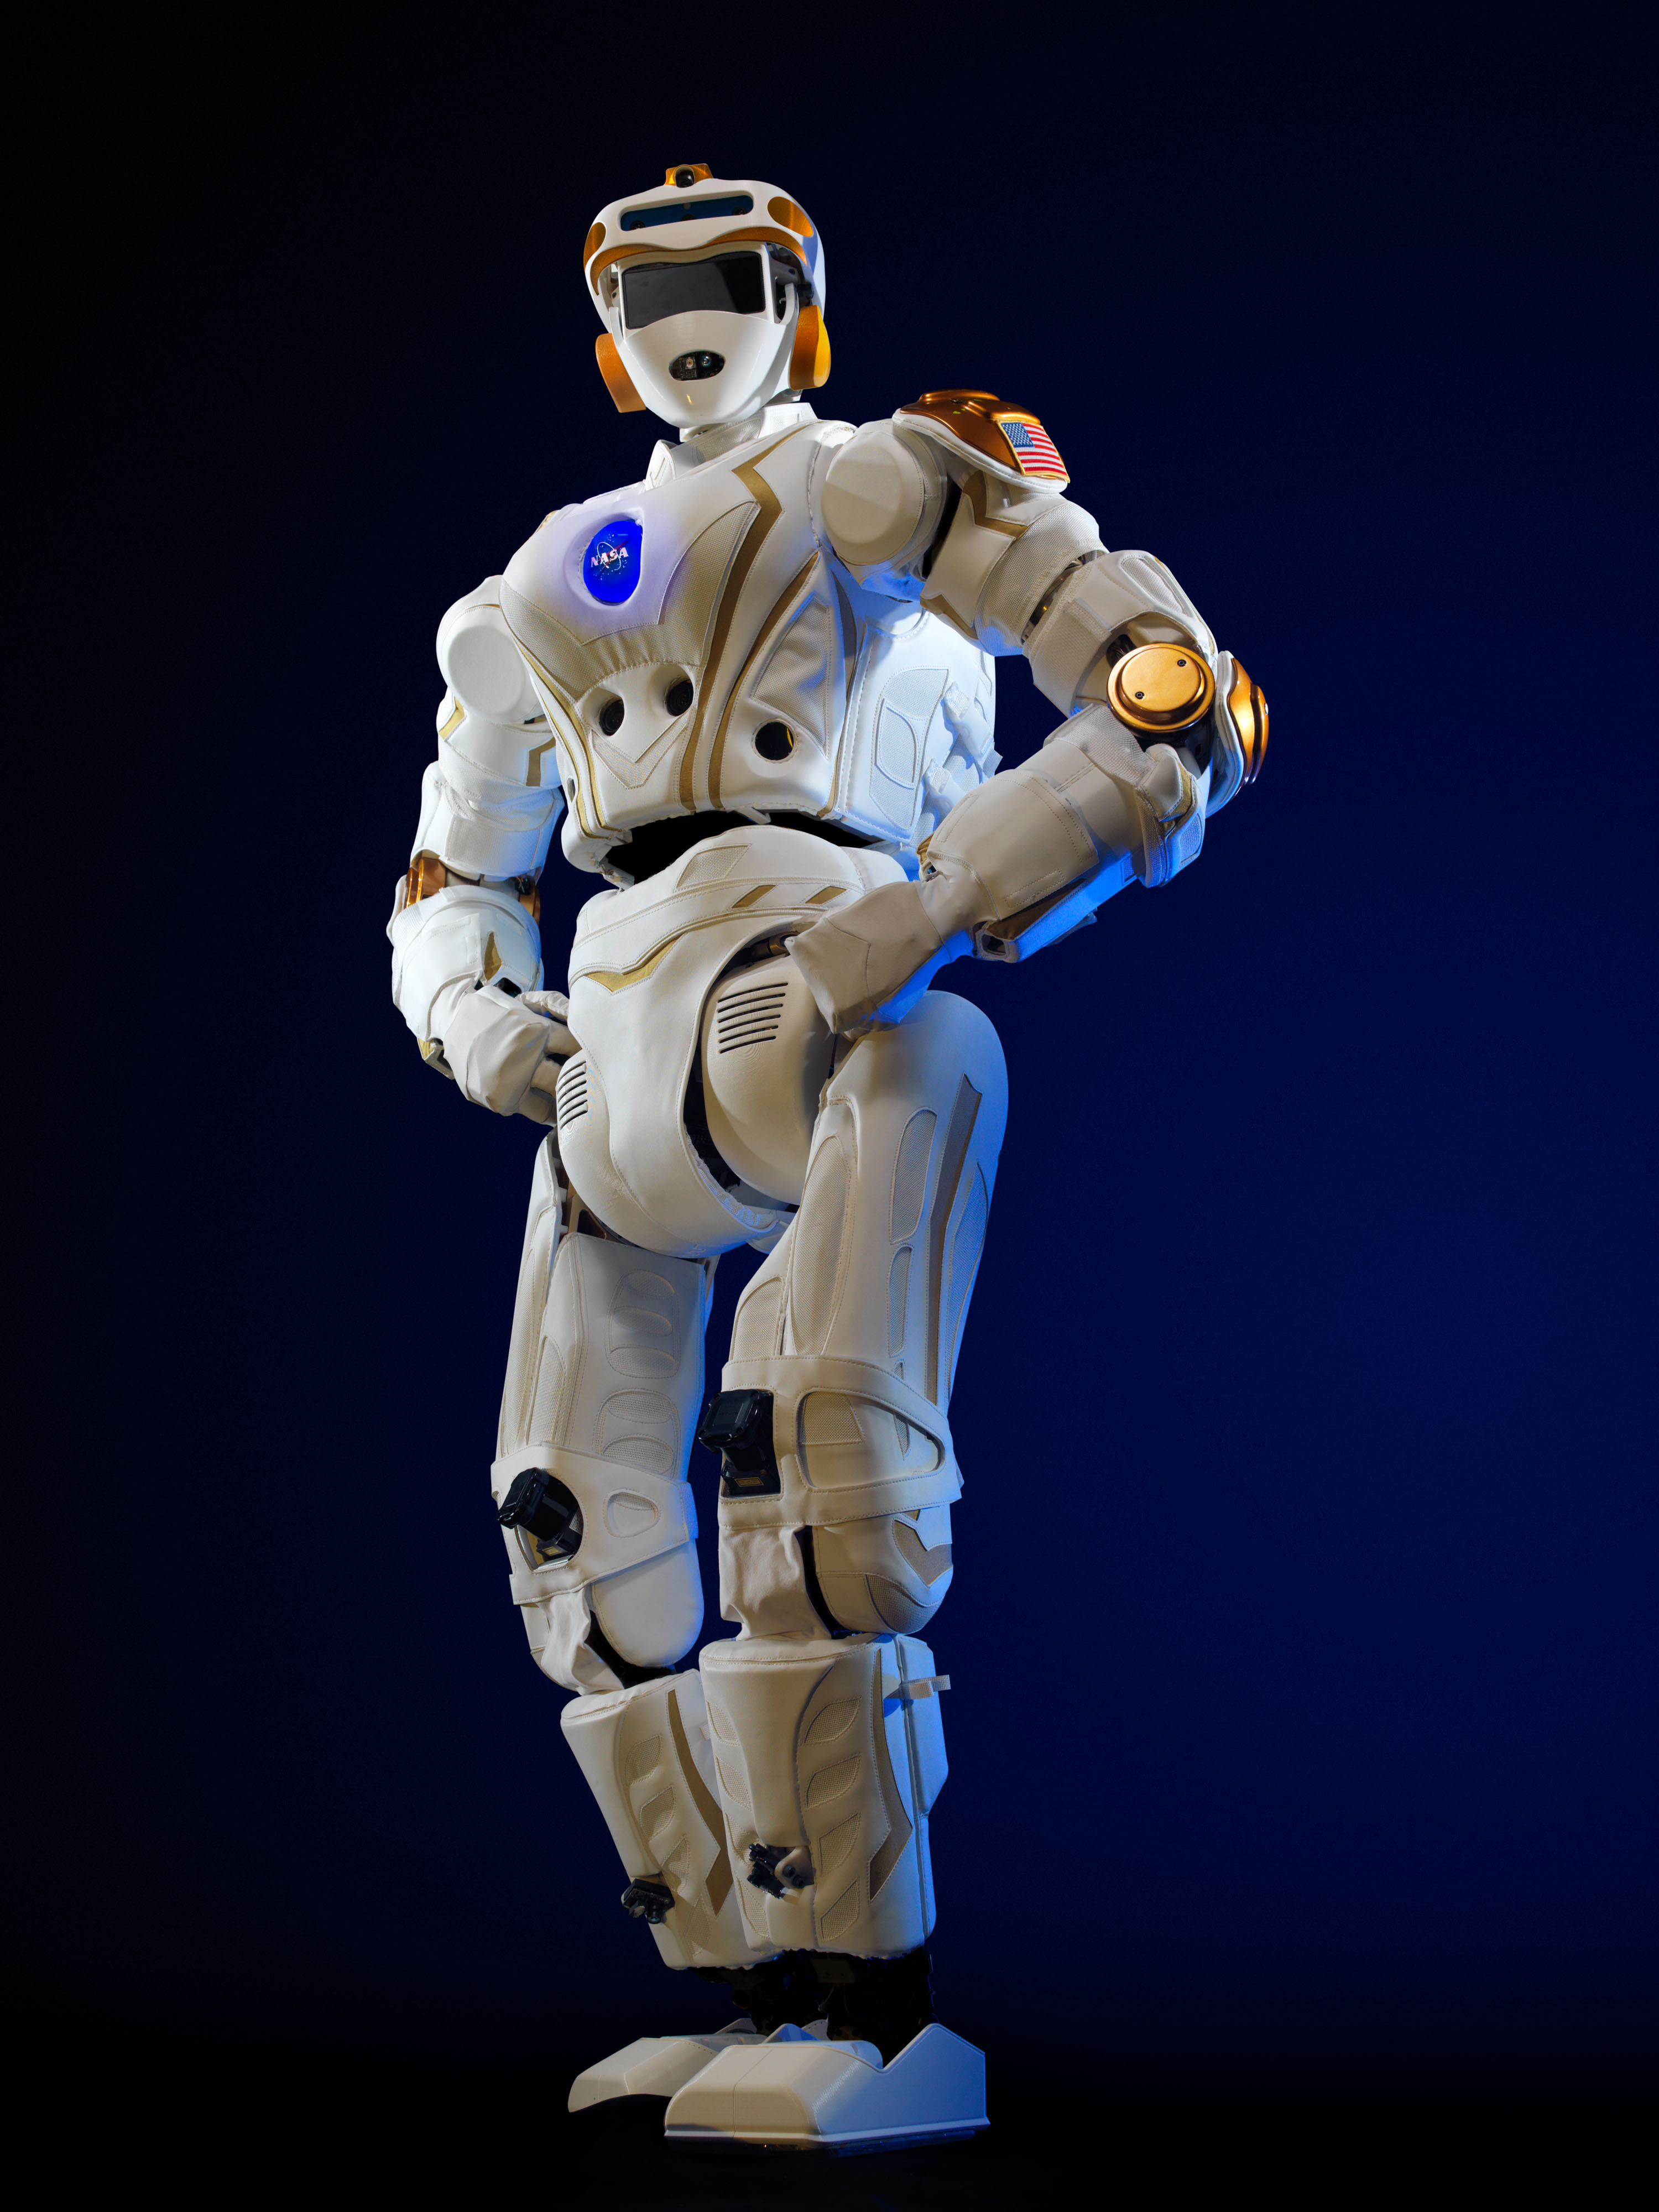
\includegraphics[width=4.2cm,height=6cm]{chapters/intro/images/valkyrie.jpg}}\quad
\end{subfigure}
\caption{Advanced Humanoid Robots}
\label{fig:hr_second}
\end{figure}

 Boston Dynamics built the hydraulics based Petman \cite{nelson2012petman} in 2012 and a series of Atlas robots from 2013. The demonstration video of Atlas in 2016 illustrated the powerful capability of the hydraulic robots by performing tasks which were impossible in the robots of the previous generation. Hydraulic actuation provides high bandwidth and high power density with the price of huge power requirements and noisy hydraulic pumps. High un-modeled friction/stiction makes it harder to control and also the high strength of actuators doesn't allow safe human-robot interaction. Series elastic actuators are also used by some laboratories in their humanoid platforms to implement torque control. The deflections in spring are measured to sense torque, and regulated to execute control on the robot. StarlETH from ETH \cite{hutter2012starleth}, IIT’s COMAN robot \cite{tsagarakis2013compliant}, Human Centered Robotics lab's Hume \cite{slovich2012hume}, IHMC’s M2V2 \cite{pratt2008design}, WALKMAN \cite{negrello2016walk}. Series elastic actuators are mechanical robust, shock absorbing and energy efficient \cite{kormushev2011bipedal} if properly controlled. Moreover, the torque control problem becomes very difficult when the actuators are very compliant and it requires precise modeling of the system dynamics.

Electrical drive units with torque sensors are still a better choice as it is necessary to perform stiff position control in some applications along with the need to have less acoustic noise and low maintenance. DLR's advanced Light Weight Robot (LWR) technology \cite{hirzinger2002dlr} for torque controlled electrical robot arms let them develop the Rollin' Justin, a humanoid upper body and the DLR biped robot \cite{ott2010development}. LWR drives were exploited in such a way it doesn't require any customization to develop a complete humanoid robot specifically for a purpose such as walking or running. TORO, a torque controlled humanoid robot with DLR-Biped legs has abilities to perform multi contact interaction and dynamic whole body motion \cite{englsberger2014overview}. The robot is equipped with torque \& position sensors in the joints including the feet and IMUs in the trunk which makes it appropriate for torque control. DURUS from SRI \cite{hereid20163d} is another robot with torque sensors and a very efficient energy transmission system with high mechanical compliance. Compliance is an important aspect to be considered when it comes to designing humanoid robots. High stiffness is required for tasks such as manipulation and for contact support whereas low stiffness is required for human-robot interaction, walking and for more dynamic activities. Ideally, we need a robot that can handle both these scenarios with ease which leaves with the idea of controlled compliance. 
\begin{figure}[!tbph]
\centering
\begin{subfigure}
[ATLAS]{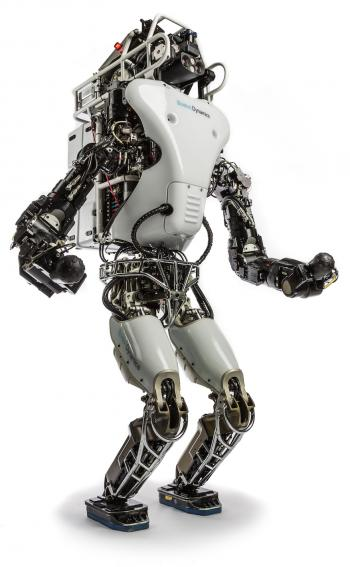
\includegraphics[width=4cm,height=6.5cm]{chapters/intro/images/atlas.jpg}}\quad
\end{subfigure}
\begin{subfigure}
[TORO]{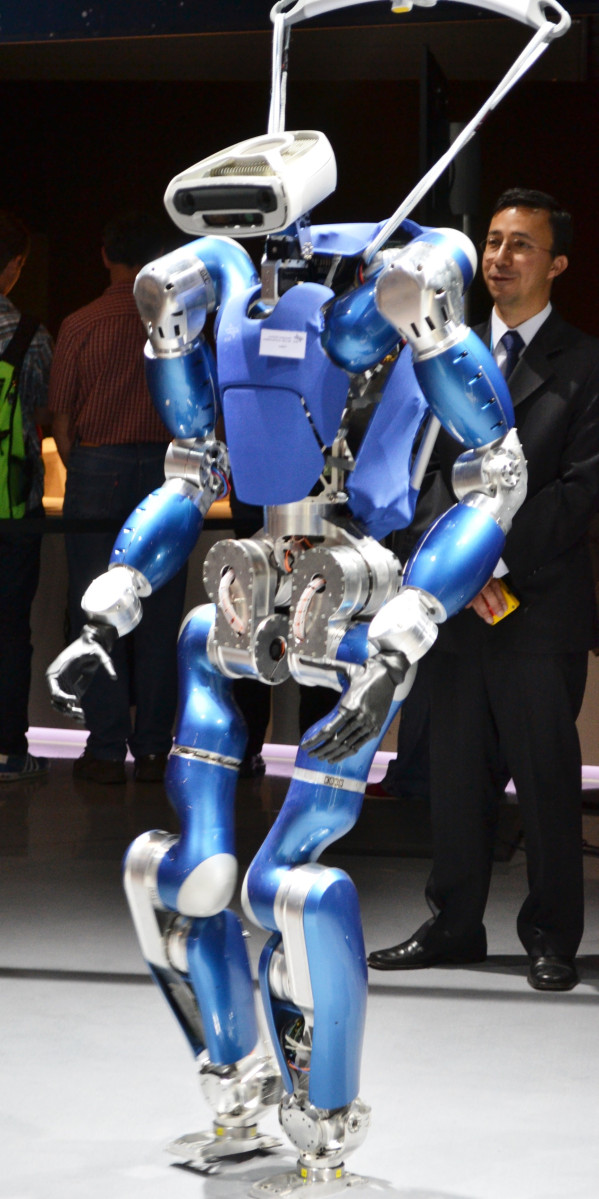
\includegraphics[width=4cm,height=6.5cm]{chapters/intro/images/toro.jpg}}\quad
\end{subfigure}
\begin{subfigure}
[TALOS]{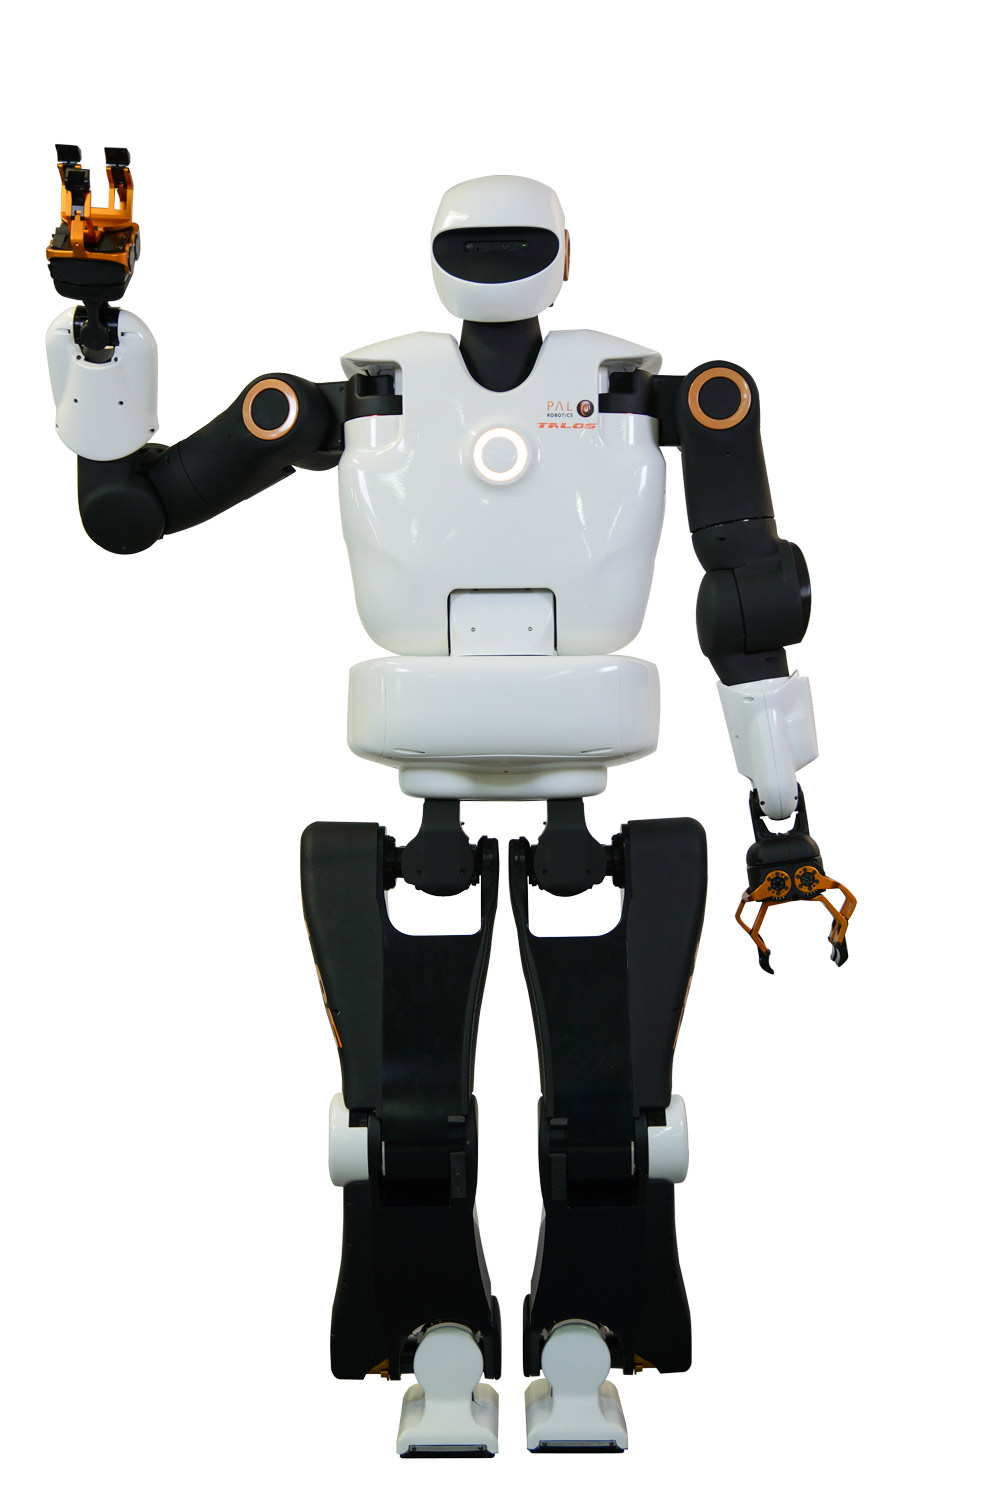
\includegraphics[width=4cm,height=6.5cm]{chapters/intro/images/talos.jpg}}\quad
\end{subfigure}
\caption{Latest Humanoid Robots}
\label{fig:hr_third}
\end{figure}

\subsection{Humanoids in Real Situations}
 Though there are a variety of humanoid robots with a lot of research going on, the applicability of those robots are quite limited. DRC competition challenged the limits of the humanoid robots by putting them in complex scenarios in dangerous environments. It is a great milestone in terms of the amount of attention the competition received and the participation of teams from different places in the world to solve problems in humanoid robotics. After filtering a lot of teams in the DRC simulation, 16 teams managed to contest in the trails. It involves a rich set of tasks that includes driving a utility vehicle, locomote across rubbles, remove debris, manipulate various tools such valves, fire hose and more. TEAM Kaist with their robot DRC-HUBO wont the contest. DRC has shown us how the robots perform in reality in spite of all the technologies working in controlled environment or in simulation. 


\begin{figure}[h]
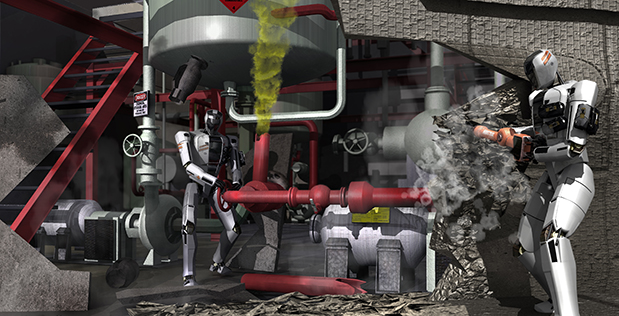
\includegraphics[scale=0.59,right]{chapters/intro/images/darpa.jpg}
\caption{DARPA Robotic Challenge}
\label{fig:darpa}
\end{figure}

The trails showed the lack of capabilities and functional robustness in task scenarios in spite of having tele-operators for guidance. The realization is that the technology is not matured enough and there are a plenty of problems to overcome. There are various aspects to these robot failures.
\begin{itemize}
    \item \textit{Robot Design}: The mechanical design of the robot has influence on the kind of failures it encounters with the environment. Walking on a flat surface is different from rough surfaces and an appropriate mechanical design is necessary to eliminate failures.

    \item \textit{Behavior Design}: The generated behaviors have to be robust to hardware failures. The kind of behaviors we choose have a big influence on the failures as well. This means robot should be able to handle variations in the task making the behavior robust. The whole body motion is also physically not depending on the external contacts. The robots usually have little or no ability to locomote using external contacts. For instance, it is very natural to hold the railings to climb up the stairs which reduces a significant amount of actuation in the joints.
    
    \item \textit{Human Robot Interaction}: When the human wants to control the robot in all the levels and switch between the modes easily, then it is not interaction anymore but intervention. Also trying to perform tasks as soon as possible puts the robot in a dynamic disadvantage.       
 
    \item \textit{Planning and Control}: Humanoid robots are redundant systems with more than 30 degrees of freedom which makes the whole body control complex. Also the pose of the robot can be only controlled indirectly by appropriate joint motions and its interaction with the environment making these robots under-actuated. 
    Constraint based inverse kinematics helps in handling control problems of humanoid robots but it is still challenging to eliminate undesired motions of the rest of the robot links while you execute the intended action in the task space. The physical interaction with the environment makes it more challenging to generate coordinated motions as it creates a variety of structural changes in the kinematics and dynamics of the robot changing the dimension of the problem. Switching control behaviors due to physical contact or joint limits or kinematic singularities challenges the limits of optimization solvers resulting in discontinuities in control. There is an ineffective use of foot torque/force sensors to close the control loop. All these problems make it easy for the robot to lose its balance.   
  
    \item \textit{Error Detection}: It is necessary to eliminate robot falls and they are mostly caused by errors generated by the system itself rather than perturbations from the environment. Detecting errors earlier can give a lot of time to take an appropriate control action to maintain balance. Though there are strategies available to handle external perturbations such as 'Push-Recovery' for example, robot generated errors are given less attention. Aborting the current behavior after detecting errors works but there is a necessity to handle them systematically. 

\end{itemize}

The above aspects shows the practical reality of the humanoid robots and the necessity of various components to function appropriately to be robust to failures. Balancing of legged robots is an essential safety constraint and the ability to handle failures is the motivation to focus on robust  balancing under inertial uncertainties of the robot model.  
